\documentclass[border=10pt]{standalone}
\usepackage{tikz}
\usepackage{amsmath}

\begin{document}
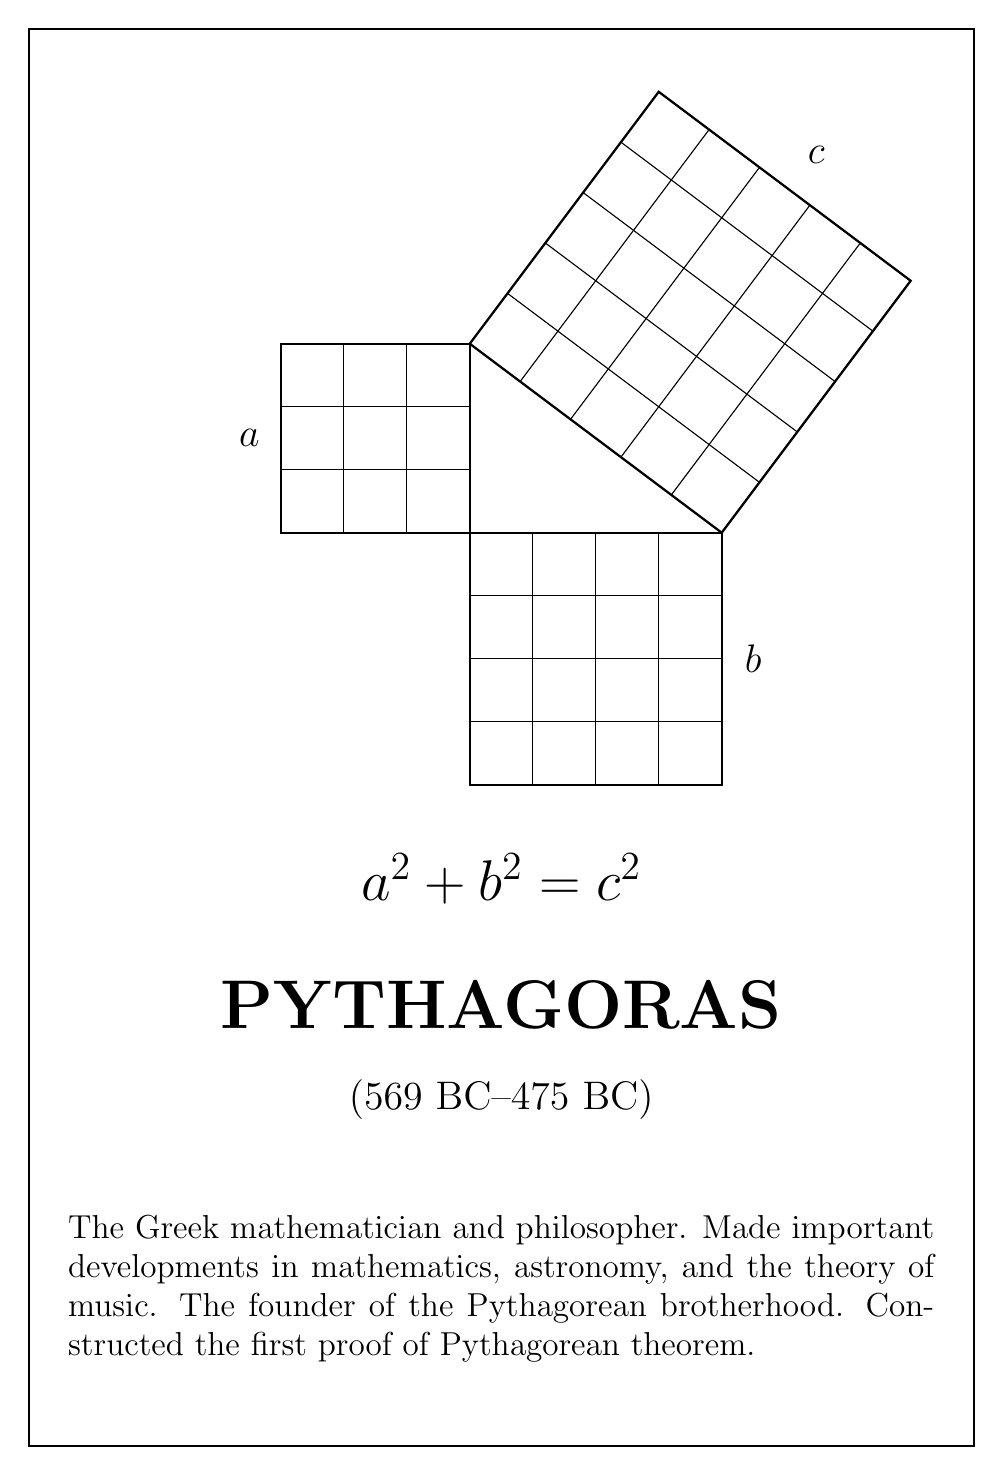
\begin{tikzpicture}[scale=0.8]

% Left square (a) - 3x3
\draw[thick] (0,0) rectangle (3,3);
\foreach \i in {0,1,2,3} {
    \draw (0,\i) -- (3,\i);
    \draw (\i,0) -- (\i,3);
}
\node at (-0.5,1.5) {\Large $a$};

% Bottom square (b) - 4x4
\draw[thick] (3,-4) rectangle (7,0);
\foreach \i in {0,1,2,3,4} {
    \draw (3,-4+\i) -- (7,-4+\i);
    \draw (3+\i,-4) -- (3+\i,0);
}
\node at (7.5,-2) {\Large $b$};

% Rotated square (c) - 5x5 at 53.13 degrees
\begin{scope}[shift={(7,0)}, rotate=53.13];
    \draw[thick] (0,0) rectangle (5,5);
    \foreach \i in {0,1,2,3,4,5} {
        \draw (0,\i) -- (5,\i);
        \draw (\i,0) -- (\i,5);
    }
\end{scope}
\node at (8.5,6) {\Large $c$};

% Formula
\node at (3.5,-5.5) {\huge $a^2 + b^2 = c^2$};

% Title
\node[font=\fontsize{40}{48}\selectfont\bfseries] at (3.5,-7.5) {PYTHAGORAS};

% Dates
\node[font=\Large] at (3.5,-9) {(569 BC--475 BC)};

% Description
\node[text width=11cm, align=justify, font=\large] at (3.5,-12) {
    The Greek mathematician and philosopher. Made important developments in mathematics, astronomy, and the theory of music. The founder of the Pythagorean brotherhood. Constructed the first proof of Pythagorean theorem.
};

% Border
\draw[thick] (-4,-14.5) rectangle (11,8);

\end{tikzpicture}
\end{document}
